\subsubsection{Increasing distance between source and destination nodes}

Figure ~\ref{fig:incrdist} shows the throughput of OPTIQ Optimization (OPT), OPTIQ Heuristic (HEU), and MPI\_Alltoallv (MPI) for disjoint, overlap and subset configurations. The experiment was done in a 2048-node partition with 256 source nodes communicating to 512 destination nodes. The set of destination nodes is chosen such that the average distance between source and destination nodes increases. Distance between 2 nodes implies the number of hops between them. The x-axes in Figures \ref{fig:incrdist_disjoint}, \ref{fig:incrdist_overlap} and \ref{fig:incrdist_subset} represent the different destination node positions. For example, in Figure \ref{fig:incrdist_disjoint}, the sources are from 0--255 and the destination position 1 refer to destination node set from node 256--767, position 2 refers to node 512--1023, position 3 refers to node 1024--1535, and destination position 4 refers to 1536--2047. The y-axes shows the throughput. We observe that the throughput of OPT and HEU increases with increasing distance in case of disjoint. This is because OPT and HEU are able to find more paths with increasing distance without increasing the maximum load on the physical links. Both Optimization and Heuristics approaches outperform MPI\_Alltoallv which uses single path for communication.
%location is moving to increase the number of hops between sources and destinations. In this experiment we show that when the distance between set of source nodes and set of destination nodes increases, we are able to find more paths while not increasing the maximum load on the physical links, thus improving performance. 
\begin{figure*}[!htbp]
        \centering
        \begin{subfigure}[b]{0.32\textwidth}
                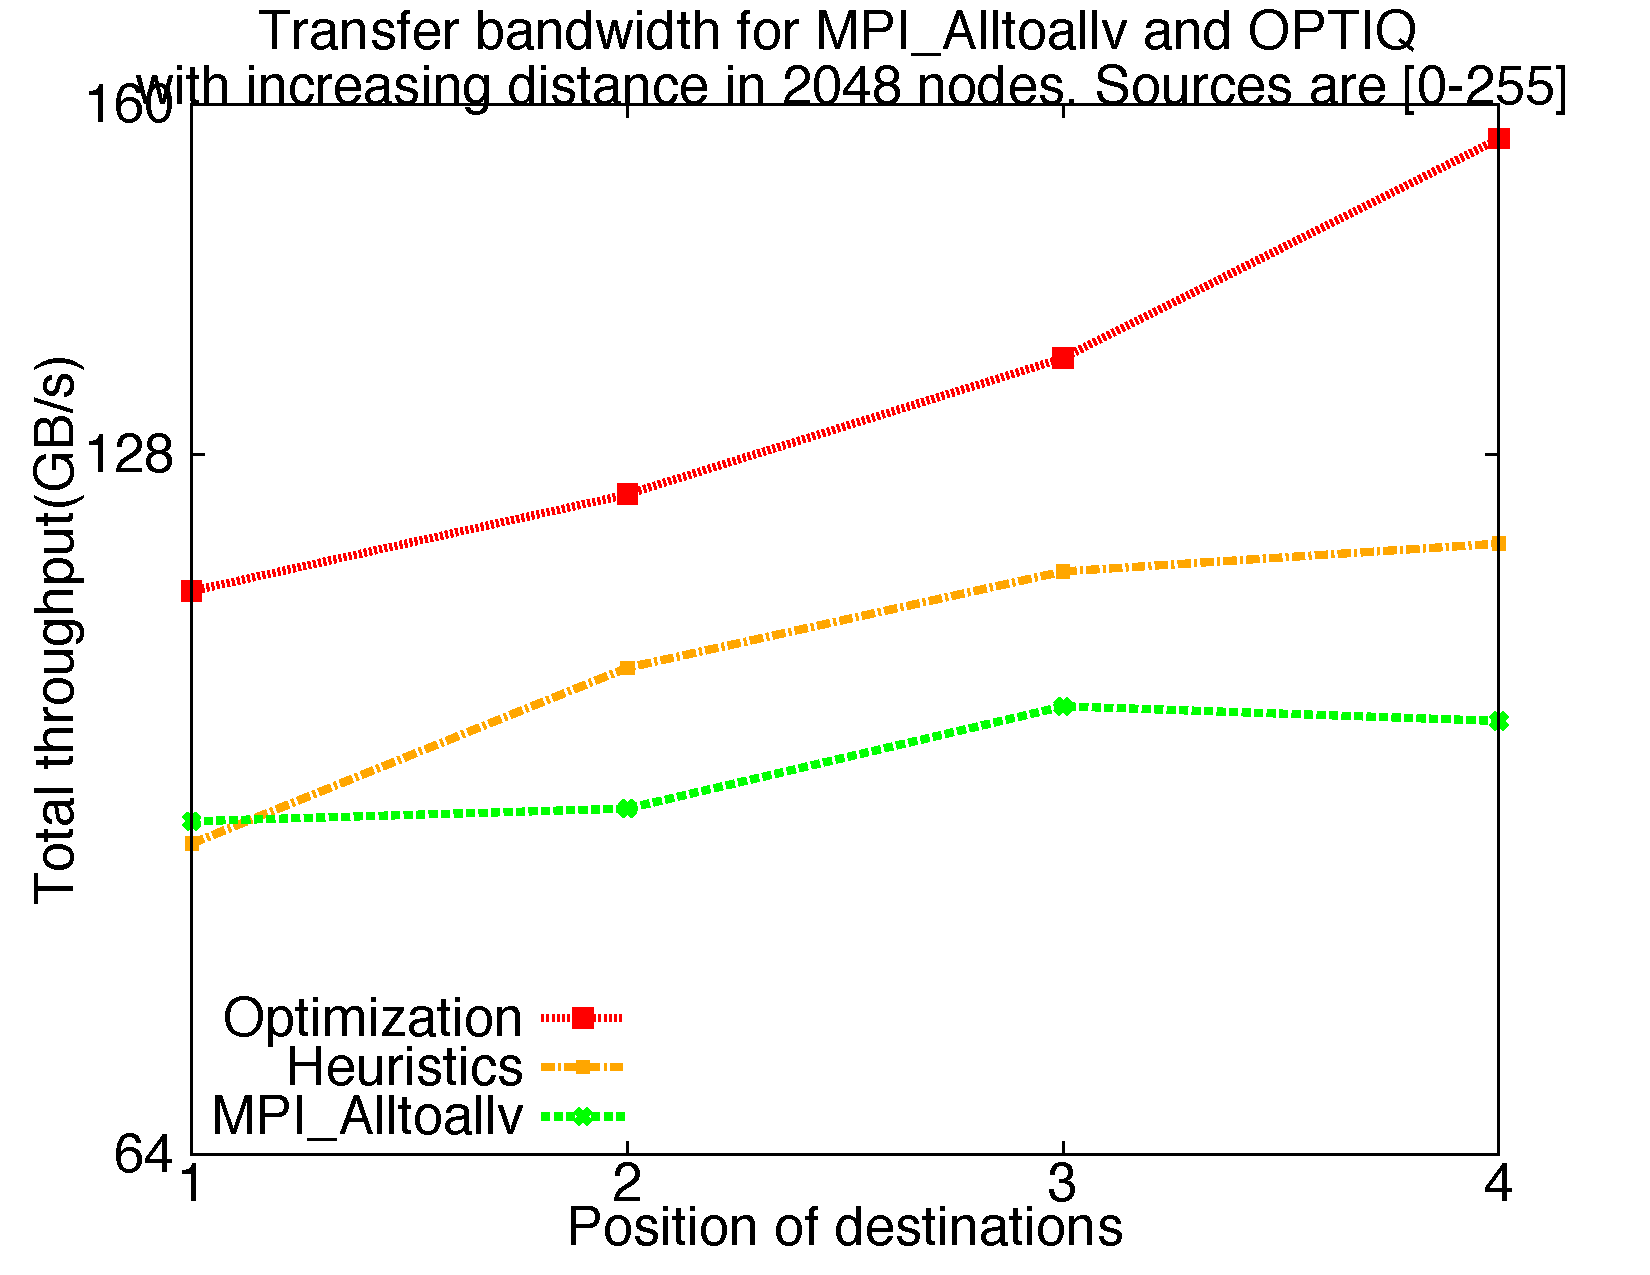
\includegraphics[width=\textwidth]{figures/incrdist_disjoint.pdf}
                \caption{Disjoint}
                \label{fig:incrdist_disjoint}
        \end{subfigure}%
        ~ %add desired spacing between images, e. g. ~, \quad, \qquad, \hfill etc.
          %(or a blank line to force the subfigure onto a new line)
        \begin{subfigure}[b]{0.32\textwidth}
                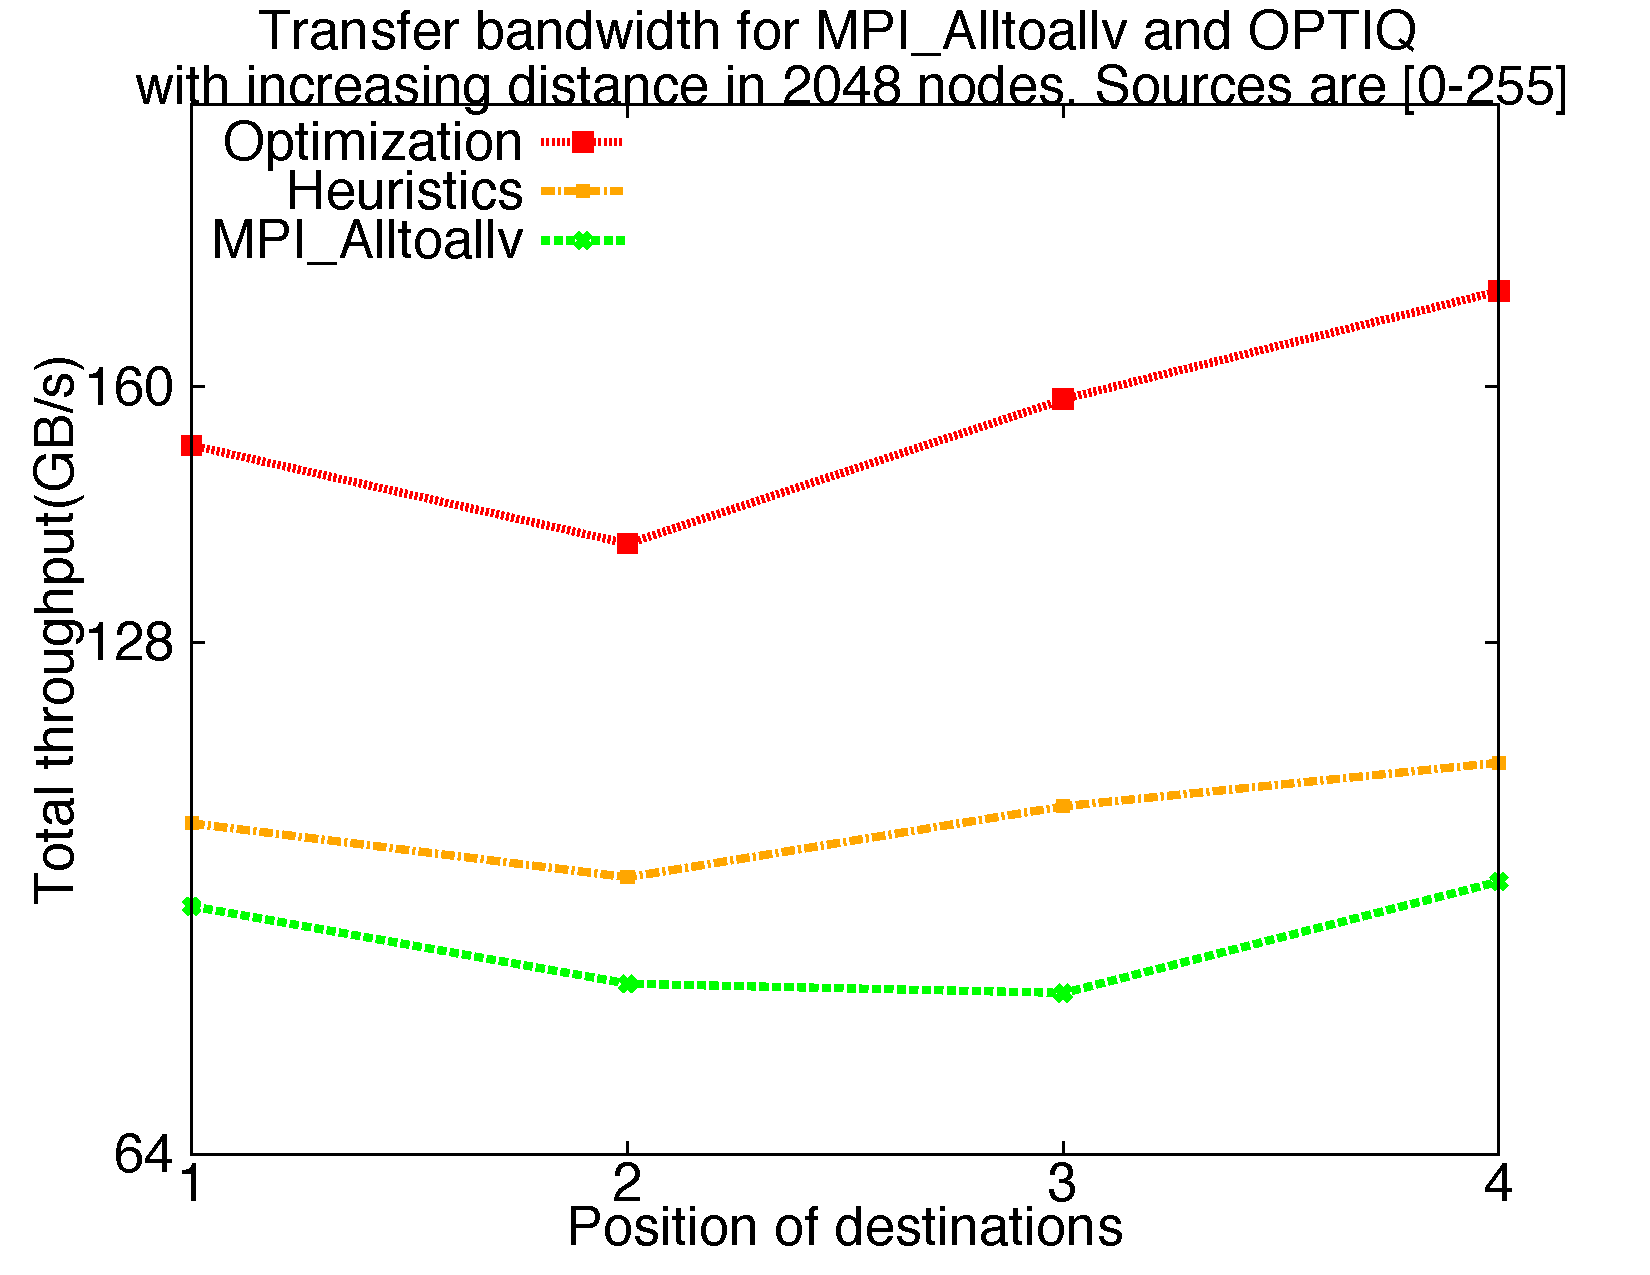
\includegraphics[width=\textwidth]{figures/incrdist_overlap}
                \caption{Overlap}
                \label{fig:incrdist_overlap}
        \end{subfigure}
        ~ %add desired spacing between images, e. g. ~, \quad, \qquad, \hfill etc.
          %(or a blank line to force the subfigure onto a new line)
        \begin{subfigure}[b]{0.32\textwidth}
                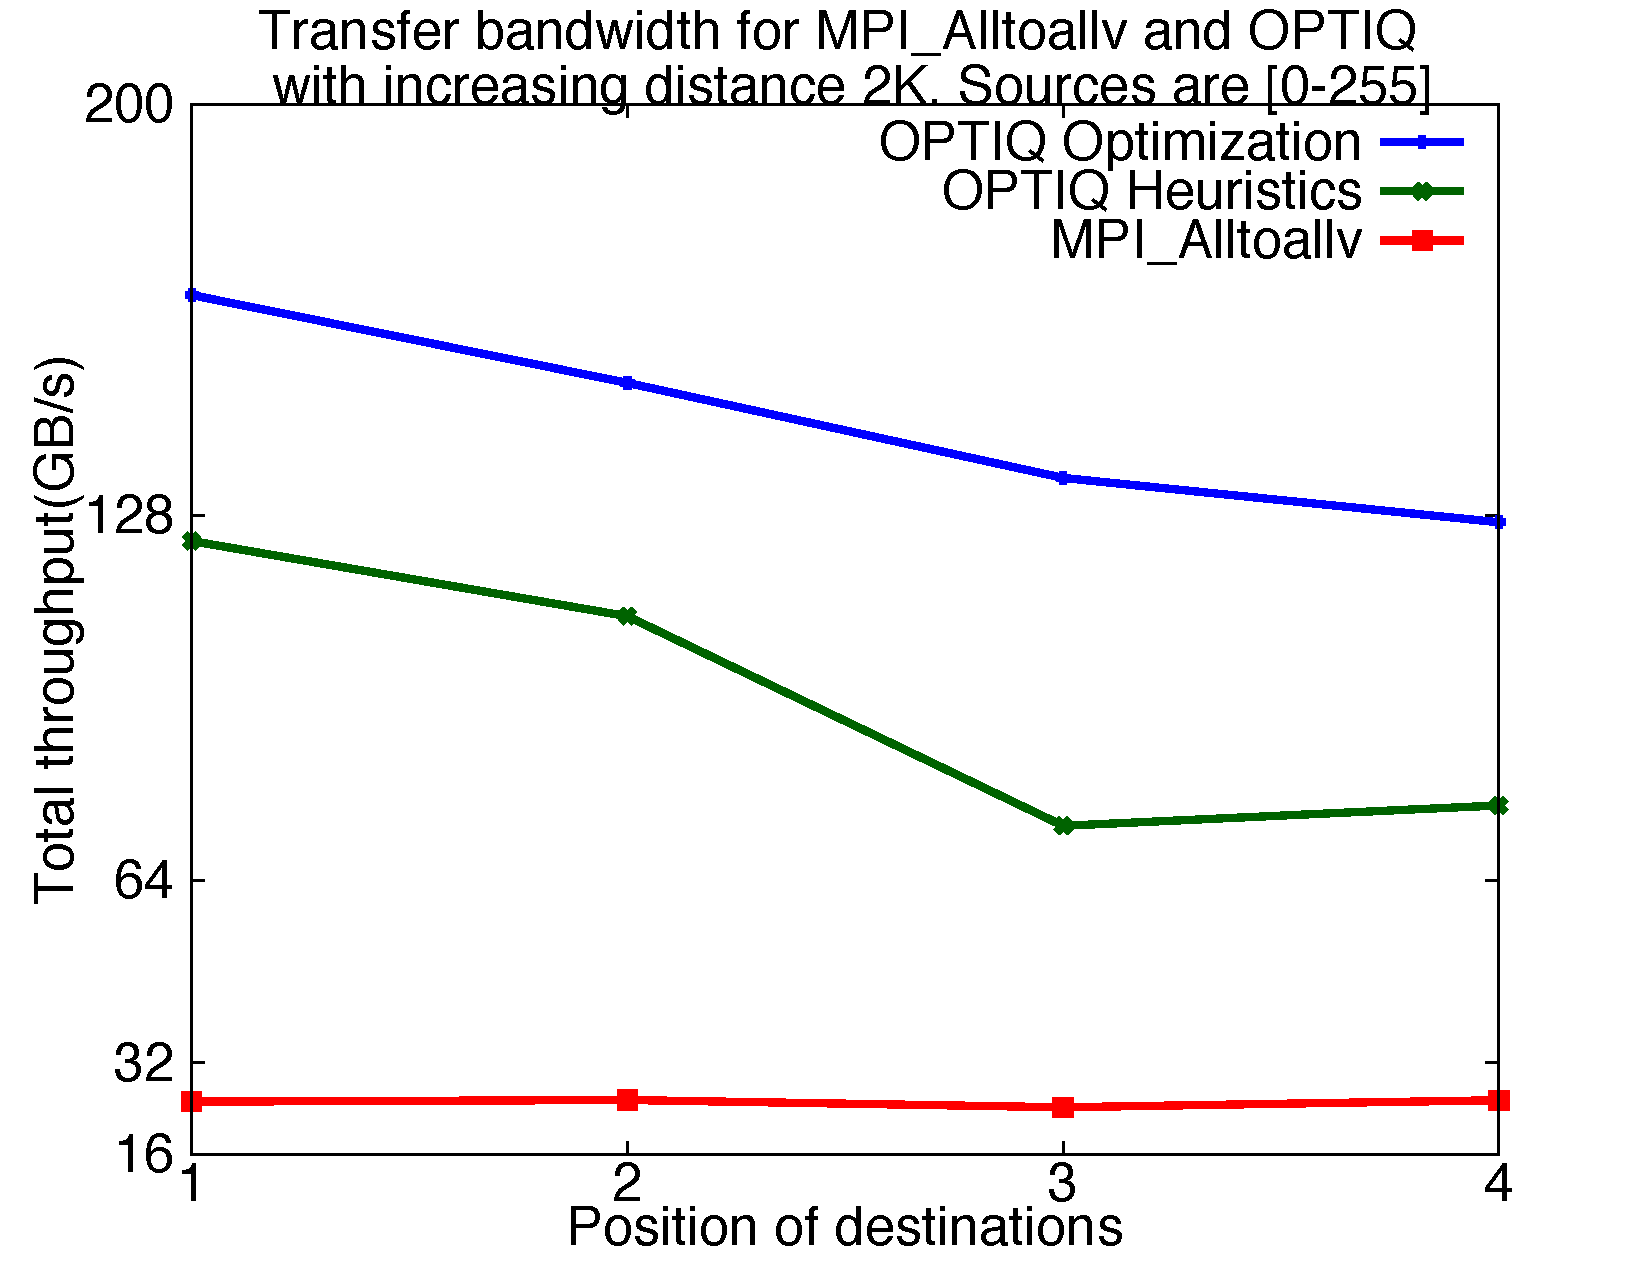
\includegraphics[width=\textwidth]{figures/incrdist_subset}
                \caption{Subset}
                \label{fig:incrdist_subset}
        \end{subfigure}
        \caption{Total data movement throughput with increasing distance between sources and destinations.}
        \label{fig:incrdist}
\end{figure*}

\begin{table*}[!htbp]
   \centering
    \begin{tabular}{| l | p{0.5cm} | p{0.5cm} | p{0.5cm} | p{0.5cm} | p{0.5cm} | p{0.5cm} |p{0.5cm} | p{0.5cm} | p{0.5cm} | p{0.5cm} |p{0.5cm} | p{0.5cm} |p{0.5cm} | p{0.5cm} |p{0.5cm} | p{0.5cm} |}
    \hline
     Positions & \multicolumn{4}{ c | }{1} & \multicolumn{4}{ c| }{2} & \multicolumn{4}{ c| }{3} & \multicolumn{4}{ c| }{4} \\ \hline
     Patterns & {Max distance} & {Avg distance} & OPT \#Paths & HEU \#Paths & Max & Avg & OPT \#Paths & HEU \#Paths & Max & Avg & OPT \#Paths & HEU \#Paths & Max & Avg & OPT \#Paths & HEU \#Paths \\ \hline
     Disjoint & 14 & 7.50 & 1105 & 2822 & 14  & 7.50 & 1372 & 2887 & 15 & 8.50 & 1547 & 3668 & 15 & 8.50 & 1672 & 3834 \\ \hline
     Overlap & 13 & 7.25 & 2085 & 6460 & 14  & 7.69 & 2152 & 3671 & 15 & 7.88 & 2337 & 6548 & 18 & 9.59 & 2399 & 7010 \\ \hline
     Subset &  20 & 8.56 & 1840 & 3422 & 21  & 8.56 & 1639 & 3364 & 22 & 9.06 & 1594 & 3119 & 23 & 9.06 & 1477 & 3087 \\ \hline
    \end{tabular}
    \caption{Maximum (Max) and average (Avg) distance between sources and destinations and number of paths for OPT and HEU for {\em disjoint}, {\em overlap} and {\em subset} on 2048 Mira nodes.}
    %\caption{Maximum (Max) and average (Avg) distance and number of paths between sources and destinations at each position.}
    \label{table:incrdist}
\end{table*}

Table \ref{table:incrdist} shows the corresponding maximum and average distances between source and destination nodes, and the number of paths for OPT and HEU for the configurations in Figure \ref{fig:incrdist}. Number of paths for MPI is 512. In general, performance of OPT improves with higher number of paths as seen in the first row for disjoint. It can also be seen that the number of paths decreases for OPT in the case of subset which leads to decrease in throughput. HEU has more paths than OPT but due to imbalanced data distribution, throughput of HEU is lower than OPT.  
%The number of paths produced by Optimization approach are 1105, 1372, 1547 and 1672 respectively. With increasing number of paths, the hopbytes, number of copies per paths and data load per physical link decrease, thus increasing in performance as shown in Figure \ref{fig:incrdist}. The same trend is observed in the Heuristics approach.
